\section{Image Analysis System}

Implementing the design from \autoref{image_analysis_design} did reveal some interesting problems, and resulted in
some equally interesting solutions. Some of them are described in this section.

\subsection{Object Detection}
The primary purpose of the system, of course, is to analyze images to find targets for the turret. It was decided
that a simple implementation using one of \ac{opencv}'s built-in algorithms, the hough circles transform would
be a good place to start. Using the hough circles algorithm does require some preparation of the image data.
The documentation of \ac{opencv} mandates that it is used only on gray-scale images, so the first step is to
desaturate the received image.

Additionally, running hough circles on a desaturated image returns a lot of ``false positives'' from image noise. The way
this was solved, was simply to apply a gaussian blur before running the transform. The result of the transform is a
list of circles, described as ($x$, $y$, $radius$). The radius is ignored in this case. The coordinates are saved directly
to a KinectData instance, and the depth for that instance is found by looking up the coordinates in the depth data.

The analyzer then tries to match the object to any previously detected objects, in this case by linking it to the closest
existing object within a certain distance threshold. The code for this can be seen in \autoref{lst:objectdetect}. The
full source has a lot of additional error handling, but what is shown should make the flow clear.

\lstinputlisting[language=Python, caption=Object Detection, label=lst:objectdetect]{listings/detect.py}

\subsection{Conversion from Kinect data to Coordinate system}
Another interesting bit
was the conversion from a location detected by the Kinect, to a point in a 3D coordinate system. The code involved
in this can be seen in \autoref{lst:kinectconvert}. The functions on the KinectData object are preliminary conversions,
as the raw data is not very useful for position calculations: The $h$ and $v$ values are pixel coordinates, and the $depth$
is received using a formula giving more precise results at close range.

The necessary calculations are all related to triangles, and figures showing the known values $h$, $v$ and $depth$,
can be seen along with the desired values $x$, $y$ and $z$ in \autoref{fig:kinectfig},
along with the triangles they can be represented with. This means that the calculations can be done with relatively
simple trigonometric formulae.

The $h$ and $v$ values are converted to degrees by first dividing them with the resolution of the received image, getting
a number between 0 and 1, which is then multiplied by the field of view of the Kinect. The depth is converted to
millimeters. At this point the law of sines is used to find the $x$ and $y$ coordinates of the object, also in
millimeters, and with those, Pythagoras' theorem is used to calculate the $z$ coordinate.

\begin{figure}[hbtp]
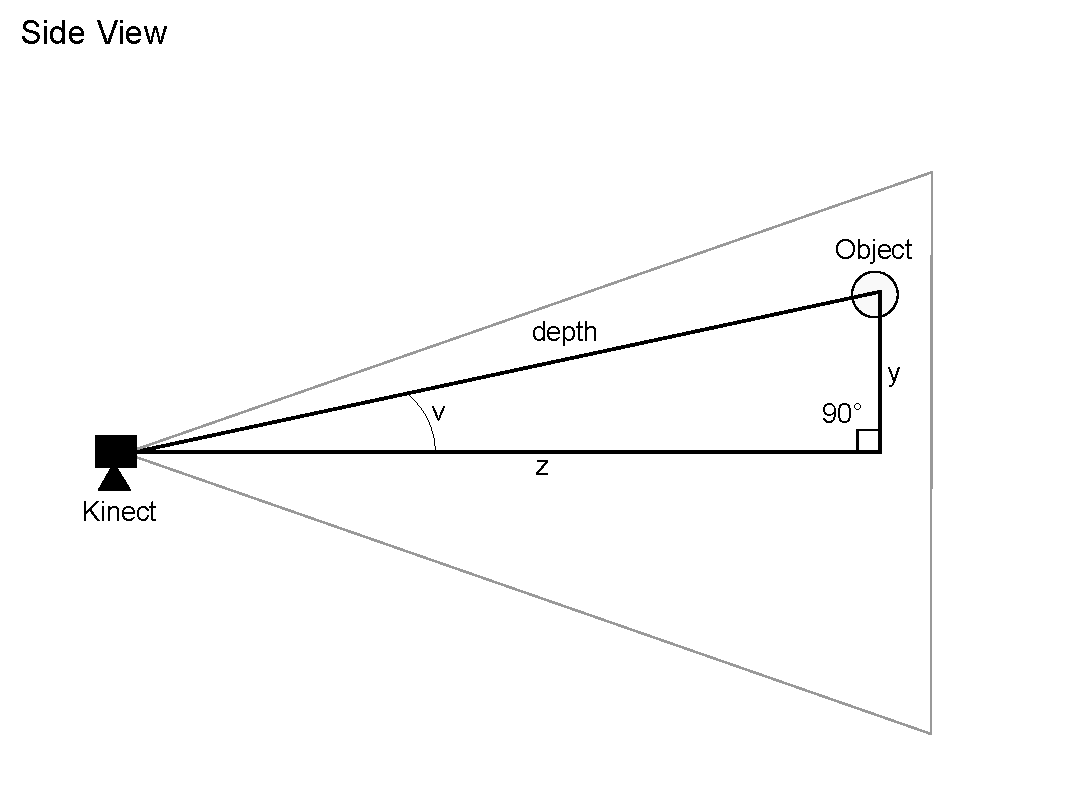
\includegraphics[width=0.90\textwidth]{img/kinectfigside.pdf}
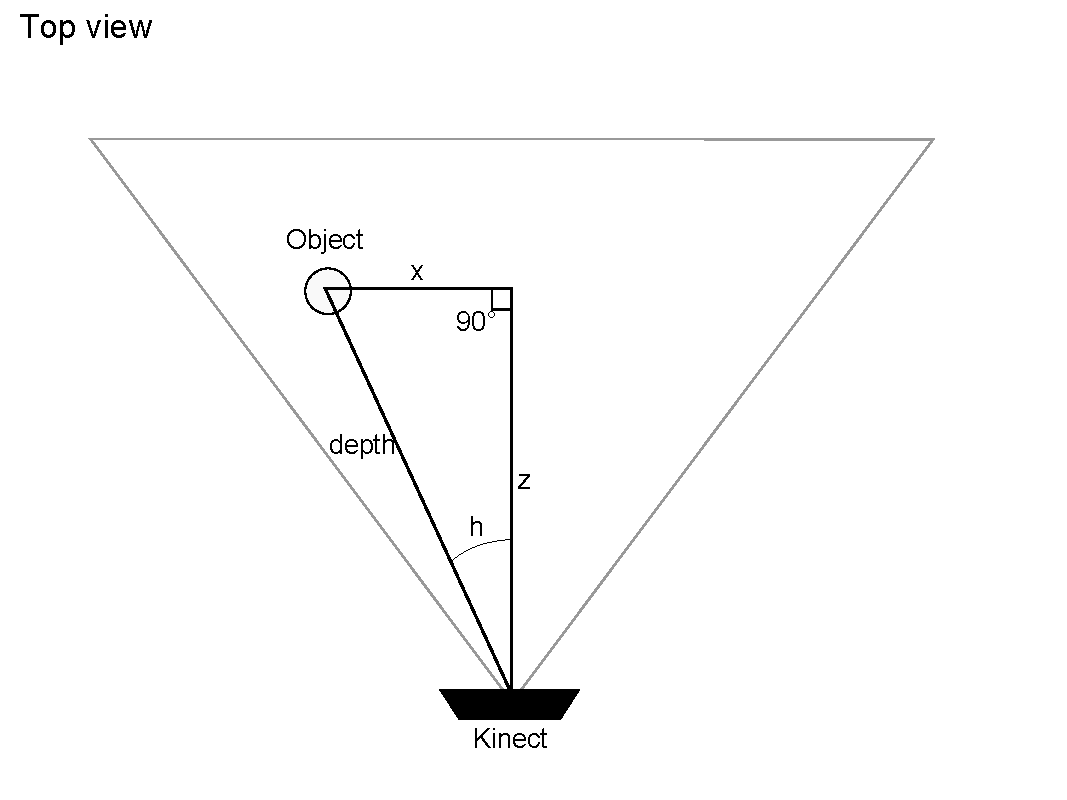
\includegraphics[width=0.90\textwidth]{img/kinectfigtop.pdf}
\caption{Overview of Kinect and Object} 
\label{fig:kinectfig} 
\end{figure}

\lstinputlisting[language=Python, caption=Kinect to Coordinate conversions, label=lst:kinectconvert]{listings/convert.py}

\subsection{Detected Object Suitability}

Another problem was determining whether a detected object was a suitable target to fire at. The solution used here is
checking whether the object has been on camera for 10 or more frames, as well as having no frames between the start and
end where it was missing. This gives a reasonable security that the object is the same, and enough data
to get a good average motion. Had this proved not to be enough, an algorithm to sort the saved positions for an object
and remove any noise could be implemented.

\subsection{Vector Arithmetic}
Several places in the application, some seen in the listings in this section, vector arithmetic is used. This is
made simpler by overloading the necessary operators on the Vector3 class, mentioned in \autoref{image_analysis_design}.
In particular, the \textbf{len} operator is overloaded to return the length of the vector, 
adding and subtracting vectors to and from each other yields the expected vector, as well does dividing or multiplying
the vector with any real number.

The subtraction is very useful, as it can be used to find the vector describing the motion between two vectors describing
points. The main use of additions is to add two vectors describing motion to each other, getting the resulting total motion.
Division is very useful for averaging a motion vector, in this case it is used to find the vector describing an object's
motion/second.
